I estimate response functions to beavers of both land used for agriculture and local environmental characteristics (namely, river level and flow intensity).

\begin{figure}
    \centering
    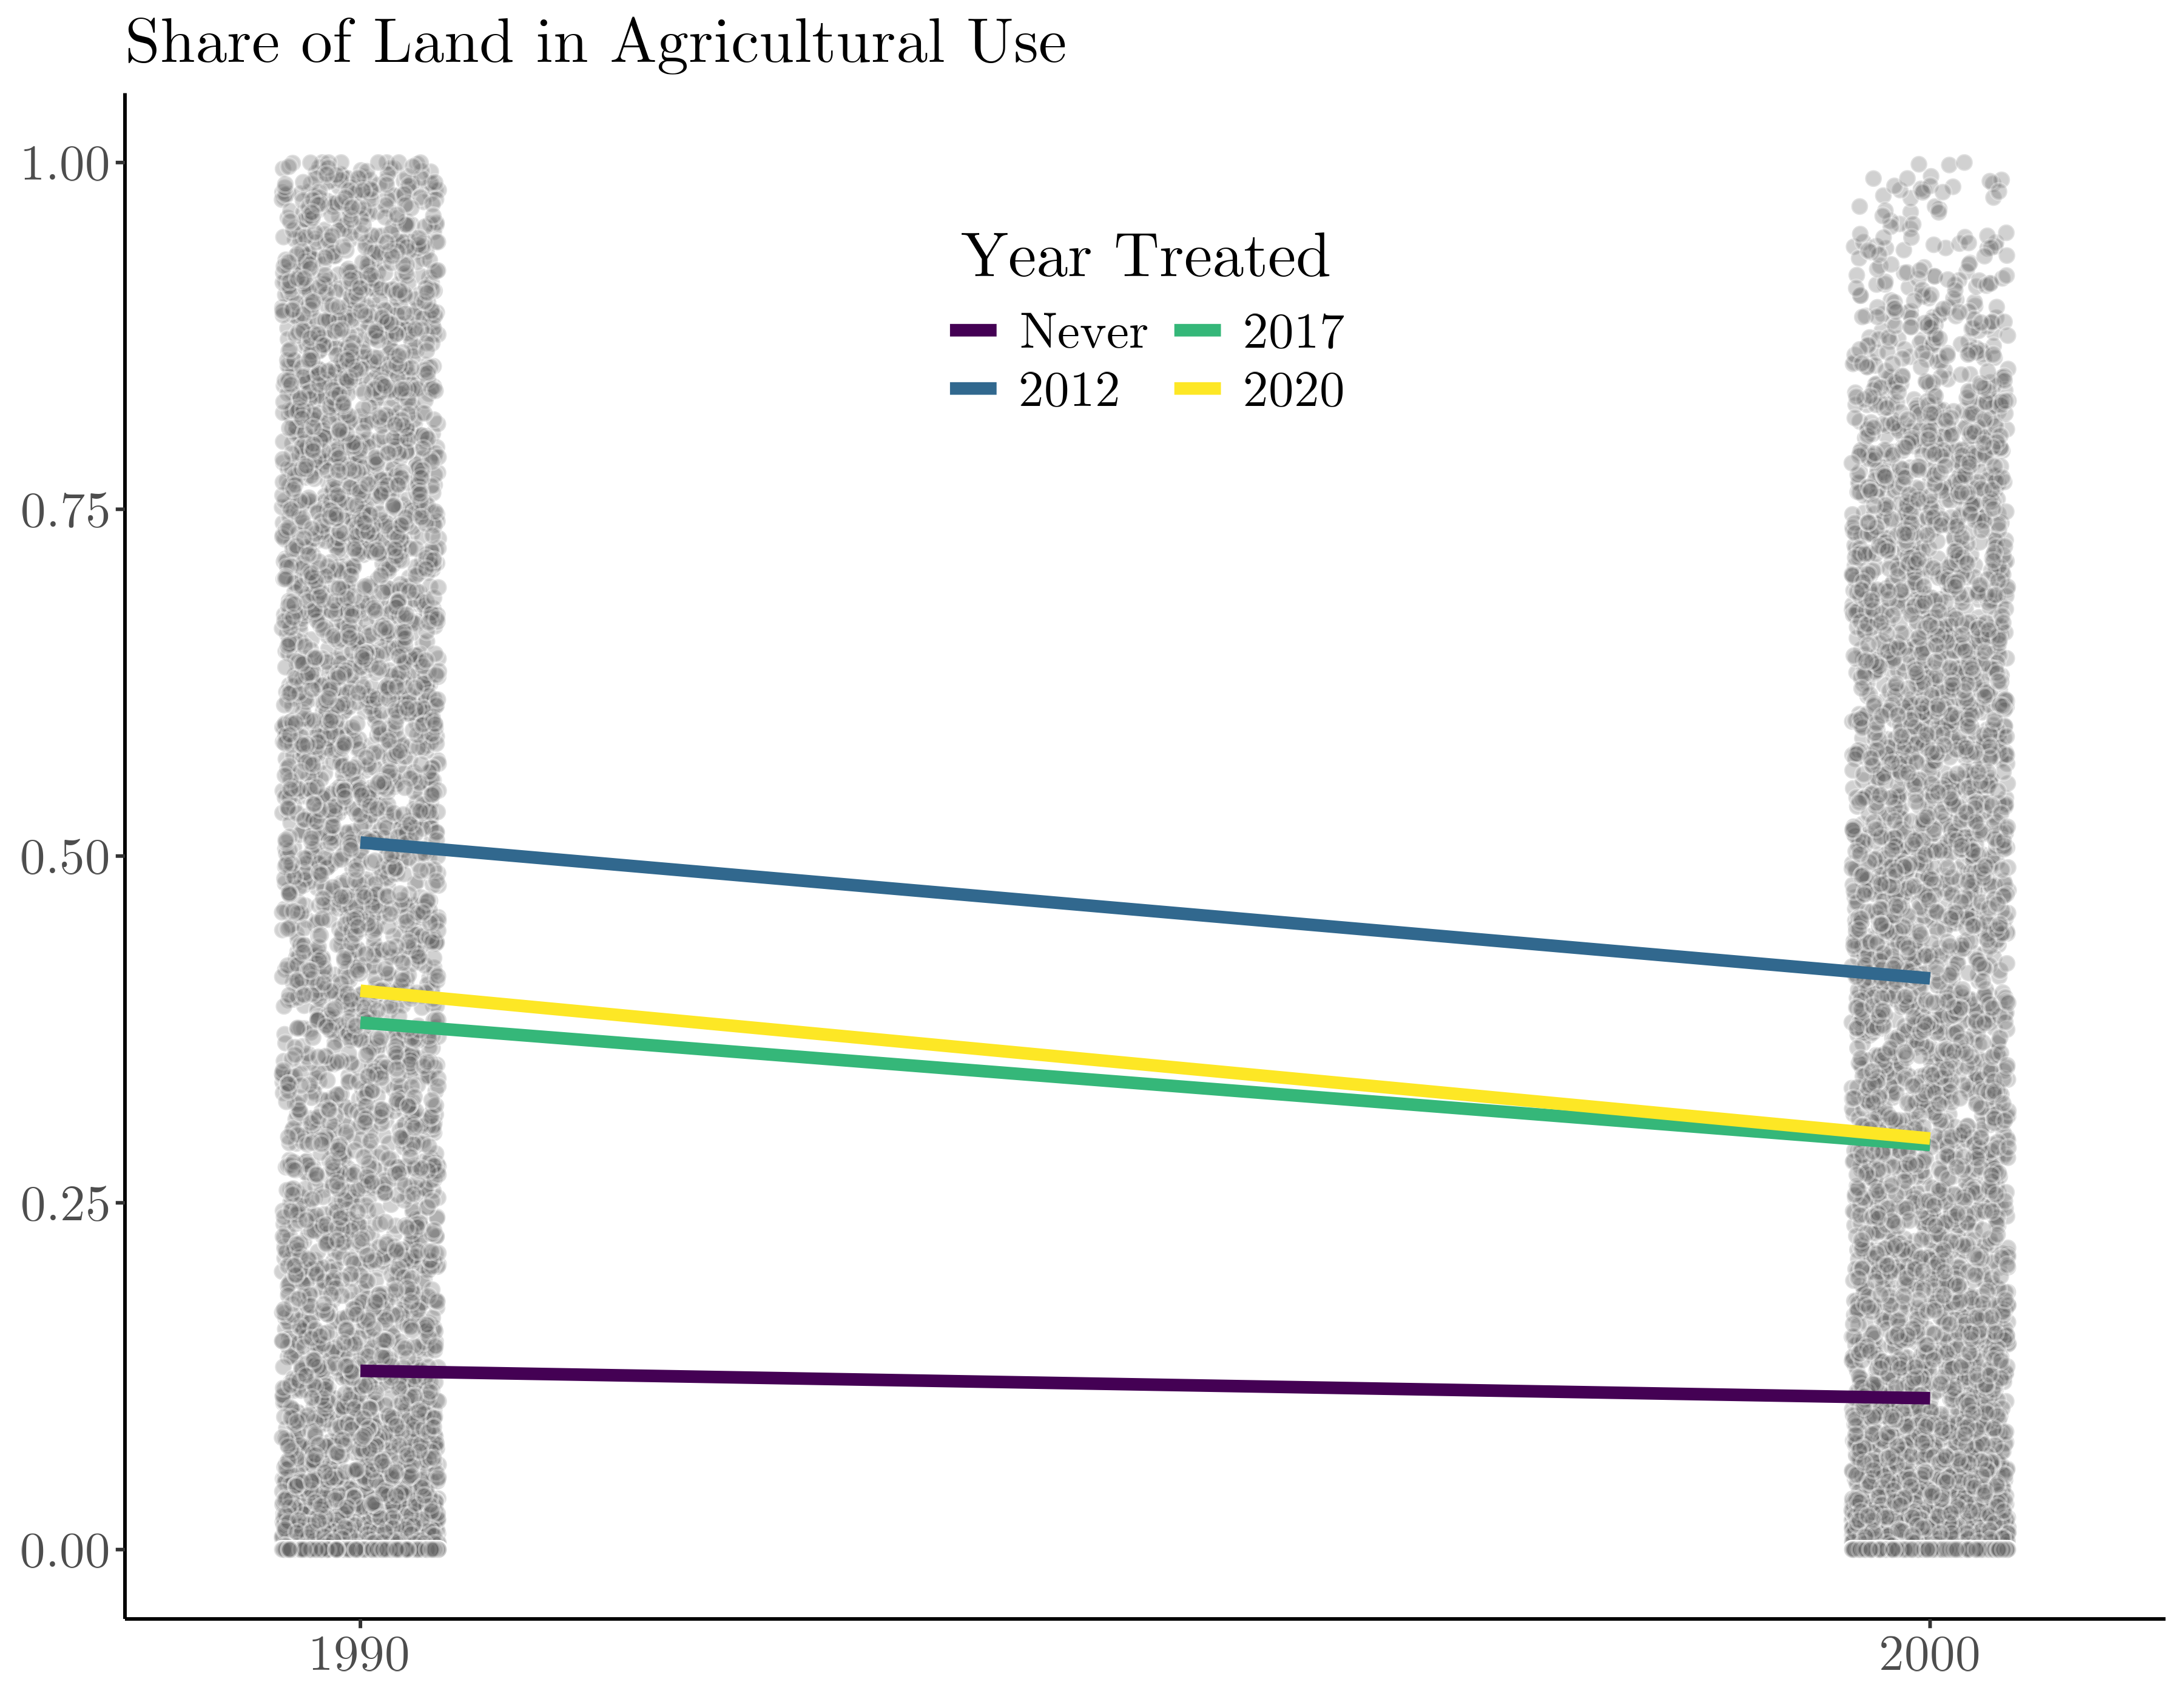
\includegraphics[width=0.7\linewidth]{output/figures/outcome_pretrends.png}
    \caption{Outcome pre-trends by treatment cohort.}
    \label{fig:outcome-pretrends}
\end{figure}

\subsection{Agricultural Land Use}

To measure the impact of beaver habitation on agricultural land use, I estimate the classic two-period difference-in-difference model

\begin{equation} \label{eq:main_beaver_eq}
y_{it} = \alpha_i + \gamma_t + \beta^{b}D_{it} + \mathbf{X}_{it} + \epsilon_{it},
\end{equation}
where $y_{it}$ is the agricultural land use outcome, $\beta^b$ is the effect of being treated by beaver presence, $D_{it}$ captures beaver treatment, $\mathbf{X}_{it}$ is a vector of time varying local environmental characteristics [\textcolor{red}{as of 28 Oct 2024, these are not yet incorporated}], and $\epsilon$ is a random error term. $\alpha_i$ and $\gamma_t$ capture grid cell and pre-and post-period fixed effects, respectively. In data aggregation, year $t \in [1990, 2000] \mapsto \gamma = 0$. For the sample including all ever-treated cohorts, $t \in [2020, 2022] \mapsto \gamma = 1$. For the sample including only 2012 and 2017 treated cohorts, $t \in [2017, 2022] \mapsto \gamma = 1$. For the sample including only 2012-treated cohort, $t \in [2012, 2022] \mapsto \gamma = 1$. To rule out one potential violation of model assumptions, in Fig. \ref{fig:outcome-pretrends}, I calculate trends in agriculture land share in the pre-treatment years for which I have land use data (1990 and 2000). All the treated cohorts display similar, slightly negative trends over this time, and while the control group is significantly less agriculture-intensive, its trend does not appear to significantly differ from those of the treated cohorts. In estimation, I test omitting cohorts and find similar results.